% \clearpage
\section{Statistical Analysis of The User Study}\label{sec:app-stats-survey}
% In this section we provide statistical details and analysis of the user study results. To begin with, we use Kullback-Leibler (KL) Divergence to compare the distributions of multi-dimensional responses between the different conditions. This allows us to measure how different the response distributions are without flattening them. The results of the KL divergence analysis is as follows:
% \begin{itemize}
%     \item There is a noticeable divergence between the distributions of balanced and unbalanced scenarios for 2-features in the familiar context (KL Divergence: 1400.53)
%     \item The KL divergence between the distributions of balanced and unbalanced scenarios for 2-features in the unfamiliar context is higher than the familiar context (KL Divergence: 2344.15). 
%     \item There is a noticeable divergence between the distributions of balanced and unbalanced scenarios for 4-features in the familiar context (KL Divergence: 324596.76)
%     \item There is a noticeable divergence between the distributions of balanced and unbalanced scenarios for 4-features in the unfamiliar context (KL Divergence: 762145.96)
% \end{itemize}


% This tells us that the distribution of balanced and unbalanced scenarios are different in all of the scenarios. The KL divergence for 4-feature scenarios are much higher than the KL divergence for 2-feature scenarios suggesting that the impact of having unbalanced features when we have more features is higher. That said, the large KL divergence for 4-feature scenarios can be a result of dimensionality. This can because in higher-dimensional spaces, distributions have more ways to differ from each other, leading to greater dissimilarity. As the number of dimensions increases, the volume of space increases exponentially, and distributions in higher dimensions tend to become more sparse, making it more likely that the two distributions differ in areas of the space.

% In Figure~\ref{fig:ks-test} we visualized the differences in investments in the most important feature using their distributions. We compare the distributions of balanced an unbalanced cases and we use the same feature for balanced scenarios (first feature in all the scenarios). The KS statistics in Table~\ref{table:KS-stats} tells us that there is a significant difference in the investment in the most important feature between balanced and unbalanced cases when the context is unfamiliar. 

% \begin{figure}[ht]
%     \centering
%     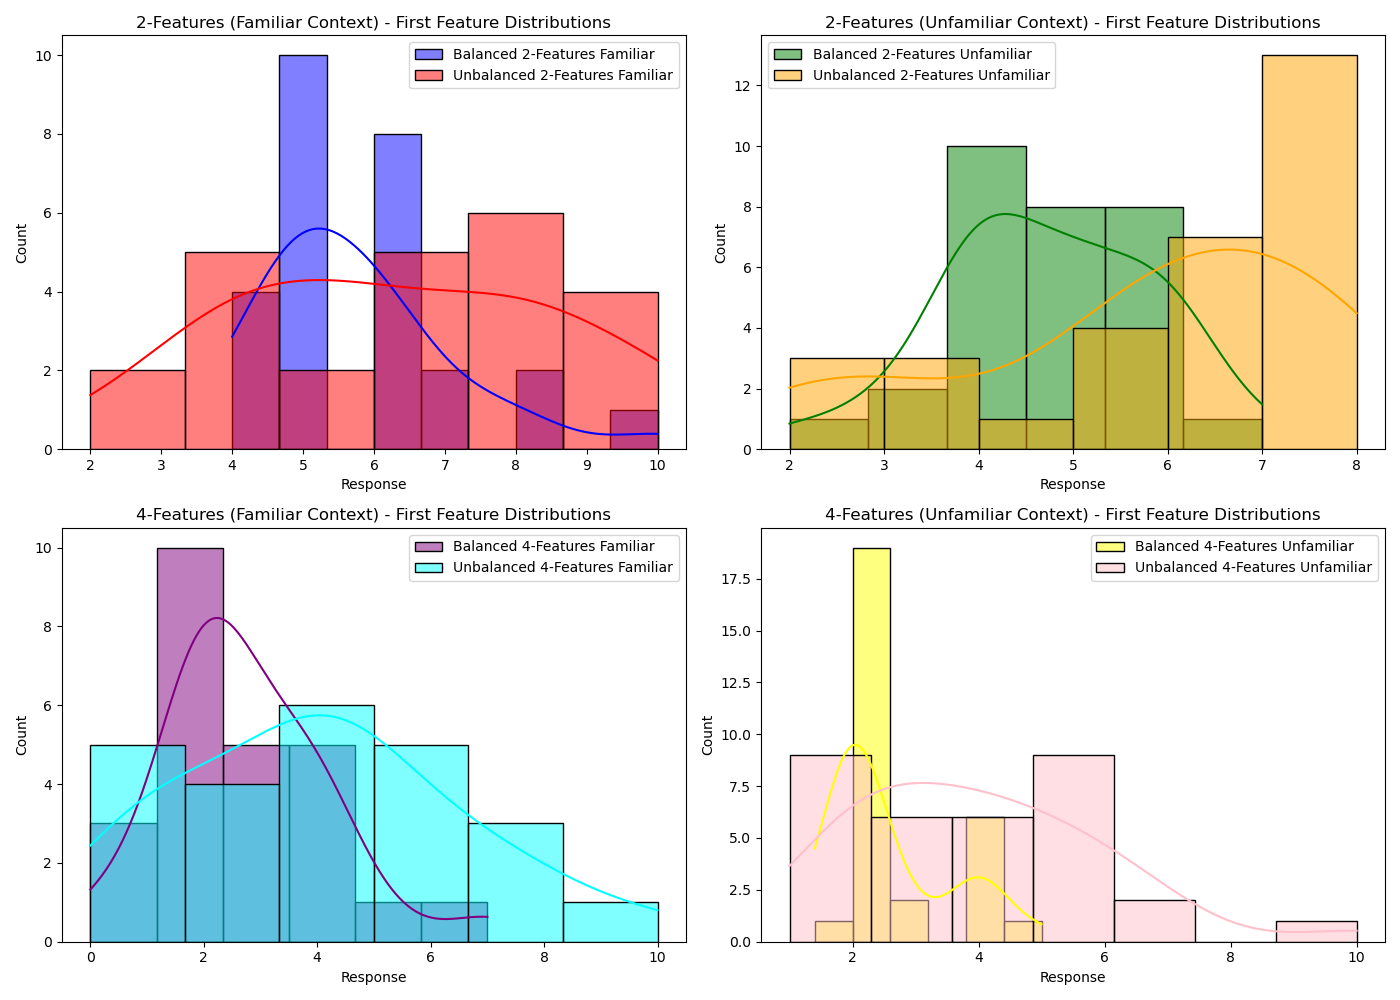
\includegraphics[width=0.7\linewidth]{Figures/ks_test_distributions.png}
%     \caption{Comparison of the distributions of the investments in the most important feature in balanced and unbalanced scenarios for 2-feature and 4-feature tasks in familiar and unfamiliar contexts.}
%     \Description[distribution comparisons]{Comparison of the distributions of balanced and unbalanced scenarios for 2-feature and 4-feature tasks in familiar and unfamiliar contexts.}
%     \label{fig:ks-test}
% \end{figure}

% \begin{table}[ht]
%     \caption{KS test statistics}\label{table:KS-stats}
%     \begin{center}
%         \begin{tabular}{lll}
%          &\textbf{KS statistic} &\textbf{P-value} \\
%         \hline \\[-4.8pt]
%         2-features (Familiar) & 0.31 & 0.15 \\
%         2-features (Unfamiliar) & 0.39 & 0.01 \\
%         4-features (Familiar) & 0.34 & 0.09 \\
%         4-features (Unfamiliar) & 0.45 & 0.002
%         \end{tabular}
%     \end{center}
% \end{table}
\begin{table*}[t]
    \caption{Mean and variance statistics}\label{table:mv-stats}
    \begin{center}
        \begin{tabular}{lllll}
         & Feature 1 ($\mu$, $\sigma^2$) & Feature 2 ($\mu$, $\sigma^2$) & Feature 3 ($\mu$, $\sigma^2$) & Feature 4 ($\mu$, $\sigma^2$)\\
        \hline \\[-4.8pt]
        2-features balanced (Familiar) & (5.74, 1.87) & (4.26, 1.87) & -- & -- \\
        2-features unbalanced (Familiar) & (6.31, 5.39) & (3.69, 5.39) & -- & -- \\
        4-features balanced (Familiar) & (2.76, 2.11) & (4.32, 3.64) & (1.68, 0.73) & (1.24, 0.77) \\
        4-features unbalanced (Familiar) & (4.06, 6.35) & (2.52, 1.81) & (1.73, 0.98) & (1.69, 2.34) \\
        2-features balanced (Unfamiliar) & (4.73, 1.25) & (5.27, 1.25) & -- & -- \\
        2-features unbalanced (Unfamiliar) & (5.74, 3.65) & (4.26, 3.65) & -- & -- \\
        4-features balanced (Unfamiliar) & (2.59, 0.90) & (3.43, 1.57) & (2.04, 0.33) & (1.94, 0.96) \\
        4-features unbalanced (Unfamiliar) & (3.97, 3.97) & (2.59, 1.21) & (1.72, 0.70) & (1.72, 1.85) 
        \end{tabular}
    \end{center}
\end{table*}

The mean and variance for investments in each scenario can be seen in Table~\ref{table:mv-stats}. As we can see the variance for unfamiliar cases are generally lower than the familiar cases. We can also see the increase in mean of the most important feature as we go from balanced cases to unbalanced cases. 

Comparing balanced and unbalanced cases, we can see higher variances in unbalanced cases. In both 2-feature and 4-feature unbalanced scenarios, we generally see a higher variance for at least one feature (often the ``most important'' feature). For Instance, in 2-features (Familiar), the variance jumps from 1.87 (balanced) to 5.39 (unbalanced) for each feature, indicating participants were much less consistent about how they allocated time when features were unbalanced. We also see greater mean differences in unbalanced cases. In unbalanced scenarios, the gap between the means of the ``most important'' and ``least important'' features tends to be larger. For example, 2-features (Familiar) goes from (5.74 vs. 4.26) in balanced (a 1.48 difference) to (6.31 vs. 3.69) in unbalanced (a 2.62 difference). 
If we compare the cases based on the number of features, we see more concentrated investments. In 2-feature scenarios, participants often put higher average investment (e.g., 5–6 hours) into the more important feature, with moderate variance. For four features, we see lower means per feature but spread out. With four features, each feature's mean is lower because participants are splitting the same total budget (10 hours) across more options. We still see unbalanced vs. balanced patterns: In 4-features balanced (Familiar), the second feature has the highest mean (4.32) but also a fairly high variance (3.64). In 4-features unbalanced (Familiar), Feature 1 jumps to a higher mean (4.06) with a large variance (6.35), suggesting participants differ widely on how much to allocate to that top feature.
